\section{Materials and Methods} \label{sec:method}

This chapter details the materials used in this work and the method proposed in this PhD thesis proposal, called \methodname. We start by describing how we gathered the datasets to train the neural network model and present some analysis of the final database. Later, we thoroughly explain our method, including the main idea behind the architecture design, its components, and the implementation details. Results and other analyses regarding the proposed work are reserved to the Chapter \ref{sec:results}.

\subsection{Datasets}

In this section, we describe the databases used by this work. First, we describe the official databases used by the FICV to benchmark algorithms that assess the \icao standard. Later, we present an expansion of this database that was used to train the proposed method. Finally, statistics about the database are detailed and discussed.

\subsubsection{FICV Dataset}

As mentioned in the literature review (see Chapter \ref{sec:literature}), one of the challenges behind the \icao standard is the lack of datasets fully labeled for all the 23 requirements. According to our previous investigation, the only dataset publicly available for research purposes is the one provided by the FICV competition for its participants. The full dataset is composed of 5588 images of 601 subjects gathered from different sources. It was built \adhoc using images from public databases, and additional images were manually acquired to cover some missing requirements. The image distribution of the FICV dataset can be seen below:

\begin{itemize}
\item 1741 images from the AR database \citep{martinez1998ar} of size 768$\times$576 pixels;
\item 1935 images from the FRGC database \citep{databaseFRGC} of sizes 1704$\times$2272 or 1200$\times$1600 pixels;
\item 291 images from the PUT database \citep{kasinski2008put} of size 2048$\times$1536 pixels;
\item 804 images artificially generated by applying ink-marked/creased, pixelation and washed out effects to compliant images from the AR database; and
\item 817 newly acquired images of size 1600$\times$1200 pixels.
\end{itemize}

Moreover, the following information is given for each image:

\begin{itemize}
\item the \textbf{coordinates of the eye corners} expressed by four pairs of $(x, y)$ coordinates (two for each eye);
\item the \textbf{compliance to the photographic and pose requirements} expressed as one of three possible values:     
    \begin{enumerate}[i]
    \item \textbf{compliant}: when a specific requirement is declared compliant for an image, it means that such image is ``OK'' for that characteristic. In theory, only fully compliant images should be considered for a later face recognition process. In the ground truth, the compliant is represented by integer 1;
    \item \textbf{non-compliant}: represented by the label 0 in the ground-truth, means the opposite of compliant. I.e., for a given image, the specific requirement is ``not-OK''; and
    \item \textbf{dummy}: used for uncertainty cases. For example, when the person wears glasses with dark tinted lenses, it is hard to evaluate whether the eyes are open even for human experts. It is represented by the integer $-1$ in the ground-truth.
    \end{enumerate}
\end{itemize}

In total, 310 images are fully compliant (i.e., compliant to all the requirements), and 5278 images have one or more requirements that are non-compliant. A representative subset of 720 images, called \ficvtest, is publicly available to the participants of the FICV competition and can be used for parameter setup and training. It contains 50 fully compliant images and 670 images not compliant to one or more characteristics. The remaining images are used as the private image set used for the benchmark of submitted algorithms. The private database is referred to as \ficvofficial by the FICV. In this thesis, we also call it the official dataset of the FICV or \fvcongoing. 

Since some of the images of \ficvtest belong to public datasets and cannot be directly distributed to third parties, only the ground-truth data of each image is provided for the participants. Nevertheless, the \fvcongoing provides a utility tool with instructions to generate the training set. Therefore, the participants must first download the images of the public datasets (i.e., AR, FRGC, and PUT) from their respective websites and then use the utility tool to produce the training set. By using this tool, however, we were able to get only 571 annotated images out of the supposed 720 images in total. We contacted the person responsible for the FICV competition, but it was informed that the remaining images belong to the set of images internally acquired, and these could not be shared.

\autoref{tab:req-dist-ficv-test} shows the distribution of images for each requirement in the \ficvtest database. It is possible to see that some requirements do not have non-compliant or dummy images (e.g., \inkmarked or \framestooheavy). Therefore, we decided to increase the \ficvtest dataset using an \adhoc approach. More details are given in the next subsection.

\begin{table}[t]
\centering
\caption{Distribution of compliant (C), non-compliant (NC), and dummy (D) images for each requirement in the \ficvtest dataset.}
\label{tab:req-dist}
\begin{tabular}{clrrr}
\hline
\textbf{Req. \#} & \multicolumn{1}{c}{\textbf{Requirement description}} & \multicolumn{1}{c}{\textbf{C}} & \multicolumn{1}{c}{\textbf{NC}} & \multicolumn{1}{c}{\textbf{D}} \\ \hline
\textbf{08} & Blurred & 515 & 31 & 25 \\
\textbf{09} & Looking away & 433 & 32 & 106 \\
\textbf{10} & Ink marked/creased & 571 & 0 & 0 \\
\textbf{11} & Unnatural skin tone & 407 & 37 & 127 \\
\textbf{12} & Too dark/light & 503 & 38 & 30 \\
\textbf{13} & Washed out & 537 & 33 & 1 \\
\textbf{14} & Pixelation & 541 & 30 & 0 \\
\textbf{15} & Hair across eyes & 523 & 12 & 36 \\
\textbf{16} & Eyes closed & 474 & 31 & 66 \\
\textbf{17} & Varied Background & 335 & 155 & 81 \\
\textbf{18} & Roll/pitch/yaw & 476 & 4 & 91 \\
\textbf{19} & Flash reflection on skin & 435 & 49 & 87 \\
\textbf{20} & Red eyes & 405 & 26 & 140 \\
\textbf{21} & Shadows behind head & 452 & 2 & 117 \\
\textbf{22} & Shadows across face & 341 & 102 & 128 \\
\textbf{23} & Dark tinted lenses & 538 & 31 & 2 \\
\textbf{24} & Flash reflection on lenses & 478 & 84 & 9 \\
\textbf{25} & Frames too heavy & 571 & 0 & 0 \\
\textbf{26} & Frame covering eyes & 477 & 29 & 65 \\
\textbf{27} & Hat/cap & 538 & 32 & 1 \\
\textbf{28} & Veil over face & 498 & 73 & 0 \\
\textbf{29} & Mouth open & 340 & 115 & 116 \\
\textbf{30} & Presence of other faces & 561 & 0 & 10 \\ \hline
\end{tabular}
\end{table}

As indicated in the FICV competition webpage, there are dependencies between some requirements. For instance, when a person is wearing veil (i.e., \veiloverface is non-compliant), the evaluation of requirement \mouthopen may be impossible. In that case, this requirement would be considered as a dummy. Therefore, we analyzed the \ficvtest dataset to figure out the dependencies between non-compliant and dummy requirements. The diagram with these dependencies can be seen in \autoref{fig:icao_dependencies}.

\begin{figure}
\centering
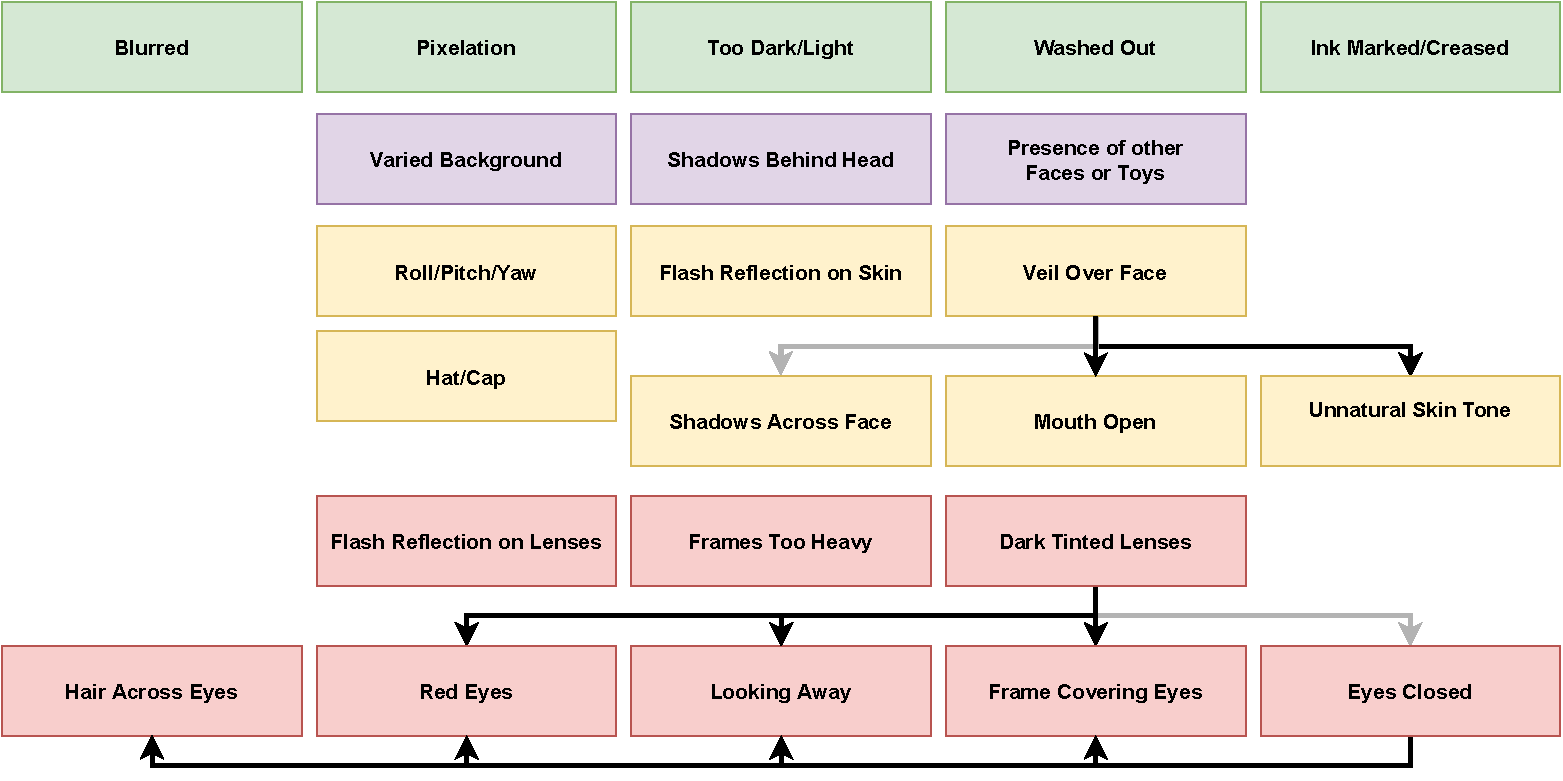
\includegraphics[width=\linewidth]{images/icao_dependencies.pdf}
\caption{Diagram of dependencies between non-compliant and dummy requirements. An arrow indicates that when the parent requirement is labeled as non-compliant, the children requirements are considered as dummy. A light gray arrow indicates that such relationship is not always true. Source: own elaboration.}
\label{fig:icao_dependencies}
\end{figure}

\subsubsection{\textit{Ad hoc} Dataset}

 Usually, \acl{dl}-based methods require a large dataset for the learning process, primarily if the training is performed from scratch. Techniques like Transfer Learning or Data Augmentation can be employed in the case of low-size datasets. However, they presume some assumptions. For example, Transfer Learning works well when the original network was trained in a similar domain compared to the new problem. Likewise, to improve results with Data augmentation, we need to have significant intraclass variance in samples. Moreover, traditional Data Augmentation does not change the distributions of labels in a dataset since the random transformations are applied uniformly. 
 
 All these problems can be found in the \ficvtest dataset. First, the \icao standard represents a unique kind of problem and, thus, Transfer Learning may not be a valid option. Although some face datasets are available for research, Neural Networks are usually trained for face recognition in these datasets. Hence, while some features learned by these networks might be helpful for ICAO, some requirements are not popular in these databases (e.g., \inkmarked) or are may be ignored by the network (like \variedbackground). Finally, Data Augmentation might not help with the \ficvtest database due to the high level of unbalancing in some requirements. Also, some transformations applied by Data Augmentation procedures could affect part of the requirements. For example, random brightness may affect the  \toodarklight requirement, and random rotations can change the angles of a face and disturb the \rollpitchyaw.
 
 With only 571 images available in \ficvtest database for all the 23 requirements, we decided to increase the dataset by following a similar procedure adopted by the FICV. Therefore, we gathered more images from the AR, FRGC, and PUT databases. We also included images from the AFW database \citep{databaseAFW} and acquired new images regarding the \icao requirements. The images were annotated by three people from our research group specially trained for this task and double-checked by two experts. In total, we ended up with a training set with 5763 images. The image distribution per dataset is defined as follows:

\begin{itemize}
\item 22 images from AFW database of sizes from 362$\times$362 to 1984$\times$1984 pixels;
\item 1368 images from AR database;
\item 50 images from PUT database;
\item 1772 images from FRGC database; and
\item 2551 newly acquired images of sizes from 976$\times$1301 to 4608$\times$3456 pixels
\end{itemize}

Our dataset has 177 fully compliant images and 5568 images with one or more non-compliant requirements. One important detail to notice is that, although the \adhoc dataset has the label dummy in the ground truth, we decided to merge dummy and non-compliant labels. We did this for two reasons. First, according to the FICV protocol, only compliant and non-compliant images are considered for benchmark of each requirement (see Section \ref{sec:fvcongoing} of Chapter \ref{sec:background}). Furthermore, the dataset imbalance is diminished by combining these two labels, and the intra-class variance of non-compliant images is increased. Therefore, it can help the network define a better decision boundary between compliant and non-compliant requirements and improve performance. Our tests corroborated such an effect. However, This decision was made aiming at the FICV competition. In other contexts, the dummy information may be relevant. Finally, the distribution of labels per requirement can be seen in Table \ref{tab:req-dist}. 

% essa decisão foi uma consequencia da competicao. Em outro contexto, o dummy pode ser importante.

To better understand the \adhoc dataset, we performed some analysis of the images and labels. Such analyses are better described in the following subsection.

% Please add the following required packages to your document preamble:
% \usepackage{graphicx}
\begin{table}[tb]
\centering
\caption{Distribution of compliant (C) and non-compliant (NC) images for each requirement in the dataset. The last column indicates the proportion of NC images for the corresponding requirement.}
\label{tab:req-dist}
\begin{tabular}{clrrr}
\hline
\textbf{Req. \#} & \multicolumn{1}{c}{\textbf{Requirement description}} & \multicolumn{1}{c}{\textbf{C}} & \multicolumn{1}{c}{\textbf{NC}} & \multicolumn{1}{c}{\textbf{NC (\%)}} \\ \hline
\textbf{08} & Blurred & 4858 & 905 & 15.7\% \\
\textbf{09} & Looking away & 3946 & 1817 & 31.5\% \\
\textbf{10} & Ink marked/creased & 5742 & 21 & 0.3\% \\
\textbf{11} & Unnatural skin tone & 2540 & 3223 & 55.9\% \\
\textbf{12} & Too dark/light & 5307 & 456 & 7.9\% \\
\textbf{13} & Washed out & 5690 & 73 & 1.3\% \\
\textbf{14} & Pixelation & 5366 & 397 & 6.9\% \\
\textbf{15} & Hair across eyes & 4252 & 1511 & 26.2\% \\
\textbf{16} & Eyes closed & 4440 & 1323 & 22.9\% \\
\textbf{17} & Varied Background & 3248 & 2515 & 43.6\% \\
\textbf{18} & Roll/pitch/yaw & 4347 & 1416 & 24.6\% \\
\textbf{19} & Flash reflection on skin & 3143 & 2620 & 45.5\% \\
\textbf{20} & Red eyes & 4531 & 1232 & 21.4\% \\
\textbf{21} & Shadows behind head & 3866 & 1897 & 32.9\% \\
\textbf{22} & Shadows across face & 4621 & 1142 & 19.8\% \\
\textbf{23} & Dark tinted lenses & 5121 & 642 & 11.1\% \\
\textbf{24} & Flash reflection on lenses & 4584 & 1179 & 20.5\% \\
\textbf{25} & Frames too heavy & 5746 & 17 & 0.3\% \\
\textbf{26} & Frame covering eyes & 4084 & 1679 & 29.1\% \\
\textbf{27} & Hat/cap & 4914 & 849 & 14.7\% \\
\textbf{28} & Veil over face & 5399 & 364 & 6.3\% \\
\textbf{29} & Mouth open & 4231 & 1532 & 26.6\% \\
\textbf{30} & Presence of other faces & 5693 & 70 & 1.2\% \\ \hline
\end{tabular}%
\end{table}

\subsubsection{\textit{Ad hoc} Dataset Analysis}

The \autoref{fig:labels_by_sample} shows the number of images with 0 or more compliant/non-compliant labels in the \adhoc dataset. As pointed out earlier, there are 177 fully compliant images (i.e., the number of non-compliant labels equals zero). Also, we can notice that most images have 2 to 6 non-compliant requirements, but there are images with up to 14 non-compliant requirements.

\begin{figure*}
\centering
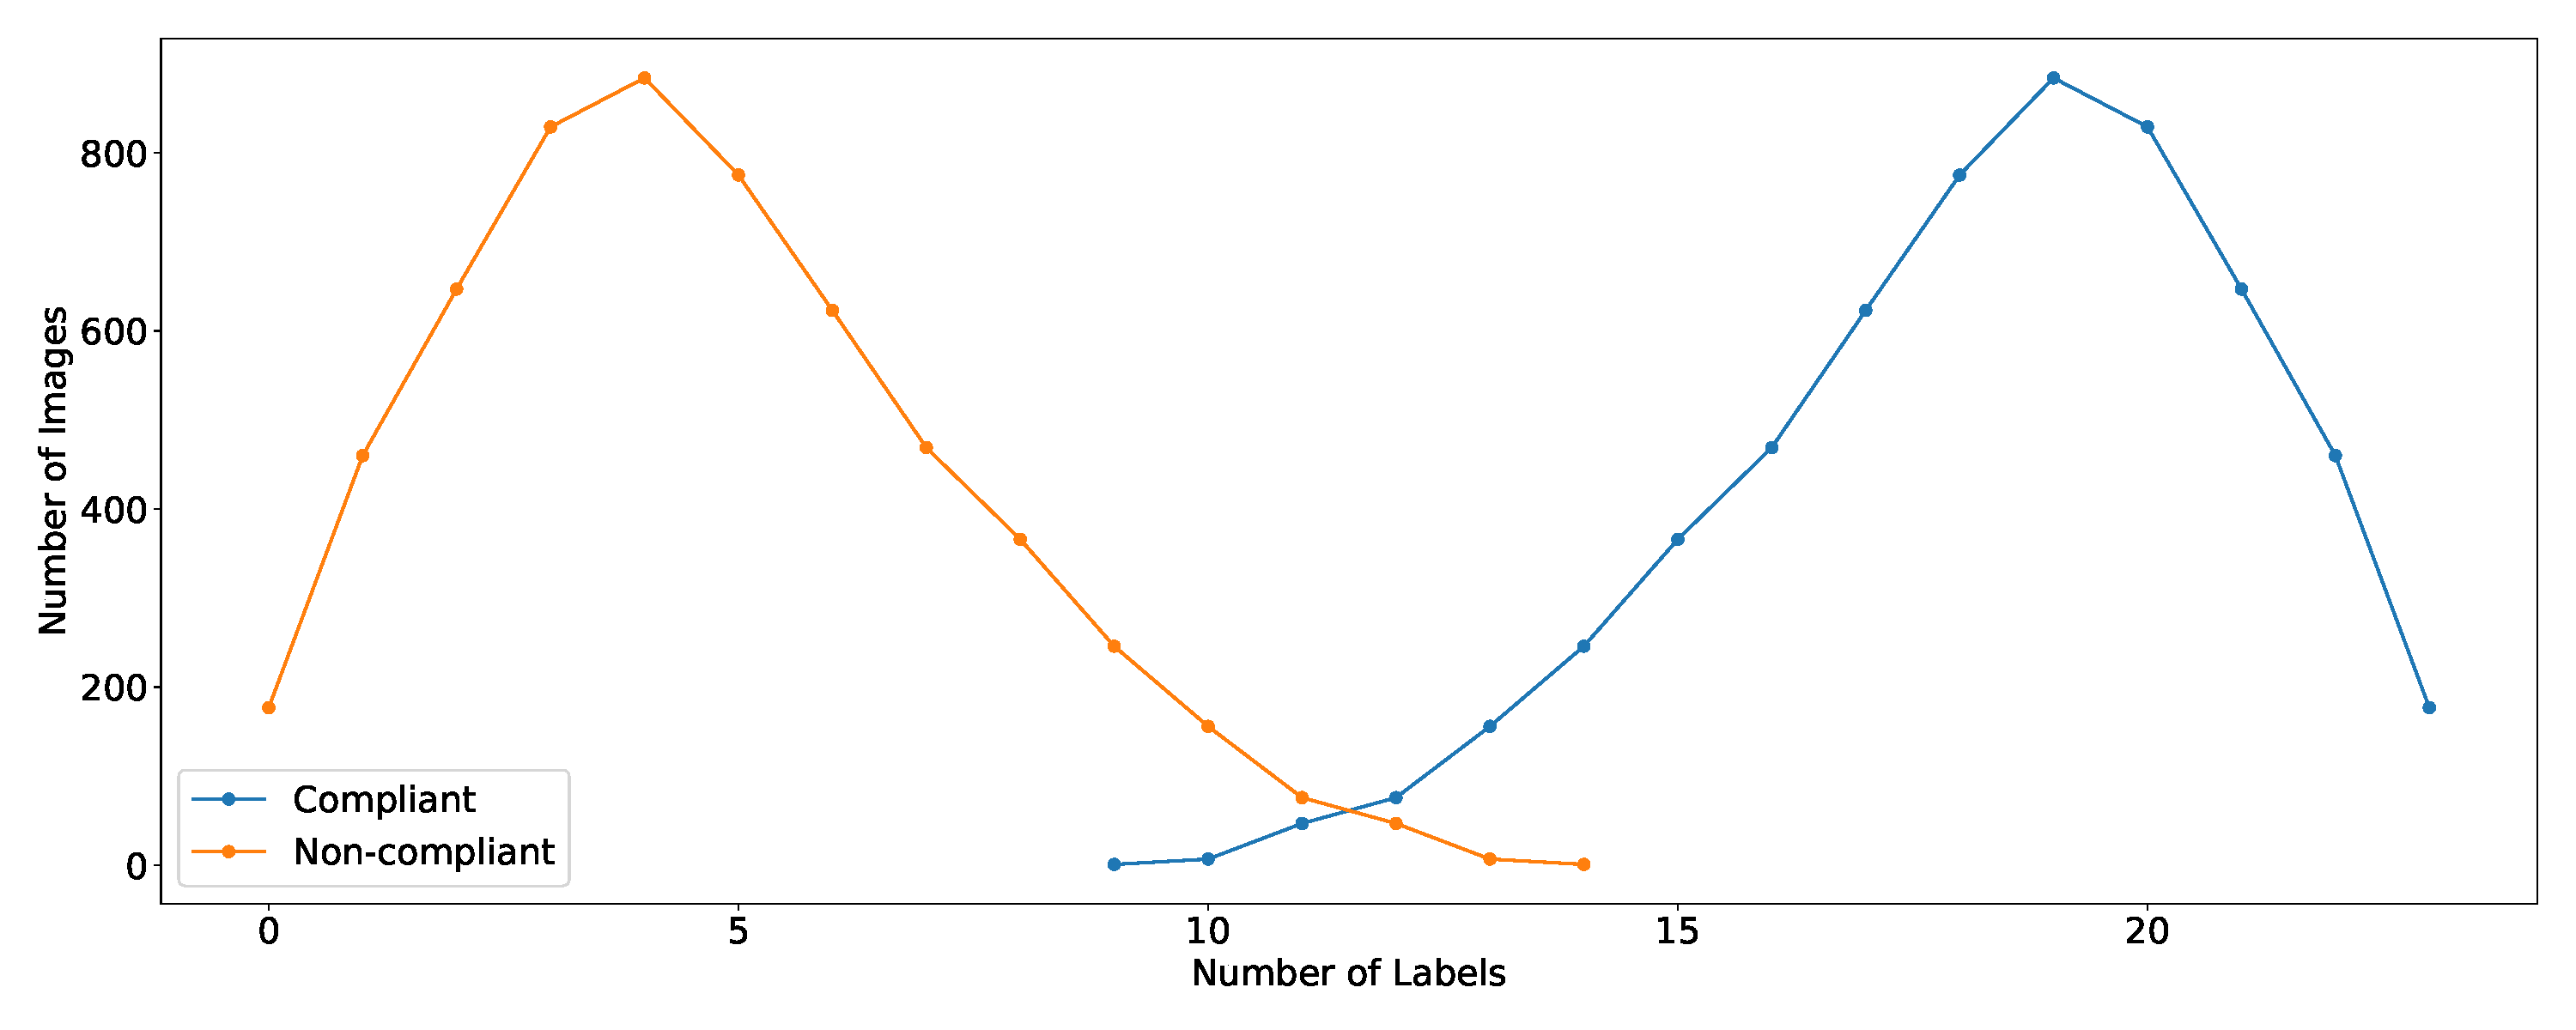
\includegraphics[width=\linewidth]{images/labels_by_sample.pdf}
\caption{Number of images according to the count of compliant/non-compliant labels. Source: own elaboration.}
\label{fig:labels_by_sample}
\end{figure*}

In \autoref{fig:reqs_distribution}, we can visualize the labels distribution by requirement presented earlier in \autoref{tab:req-dist}. As can be seen, the requirements \inkmarked, \washedout, \framestooheavy, and \otherfacesortoys are the most unbalanced ones. Also, the \unnaturalskintone is the only requirement where the number of non-compliant samples is greater than the compliant.

\begin{figure*}
\centering
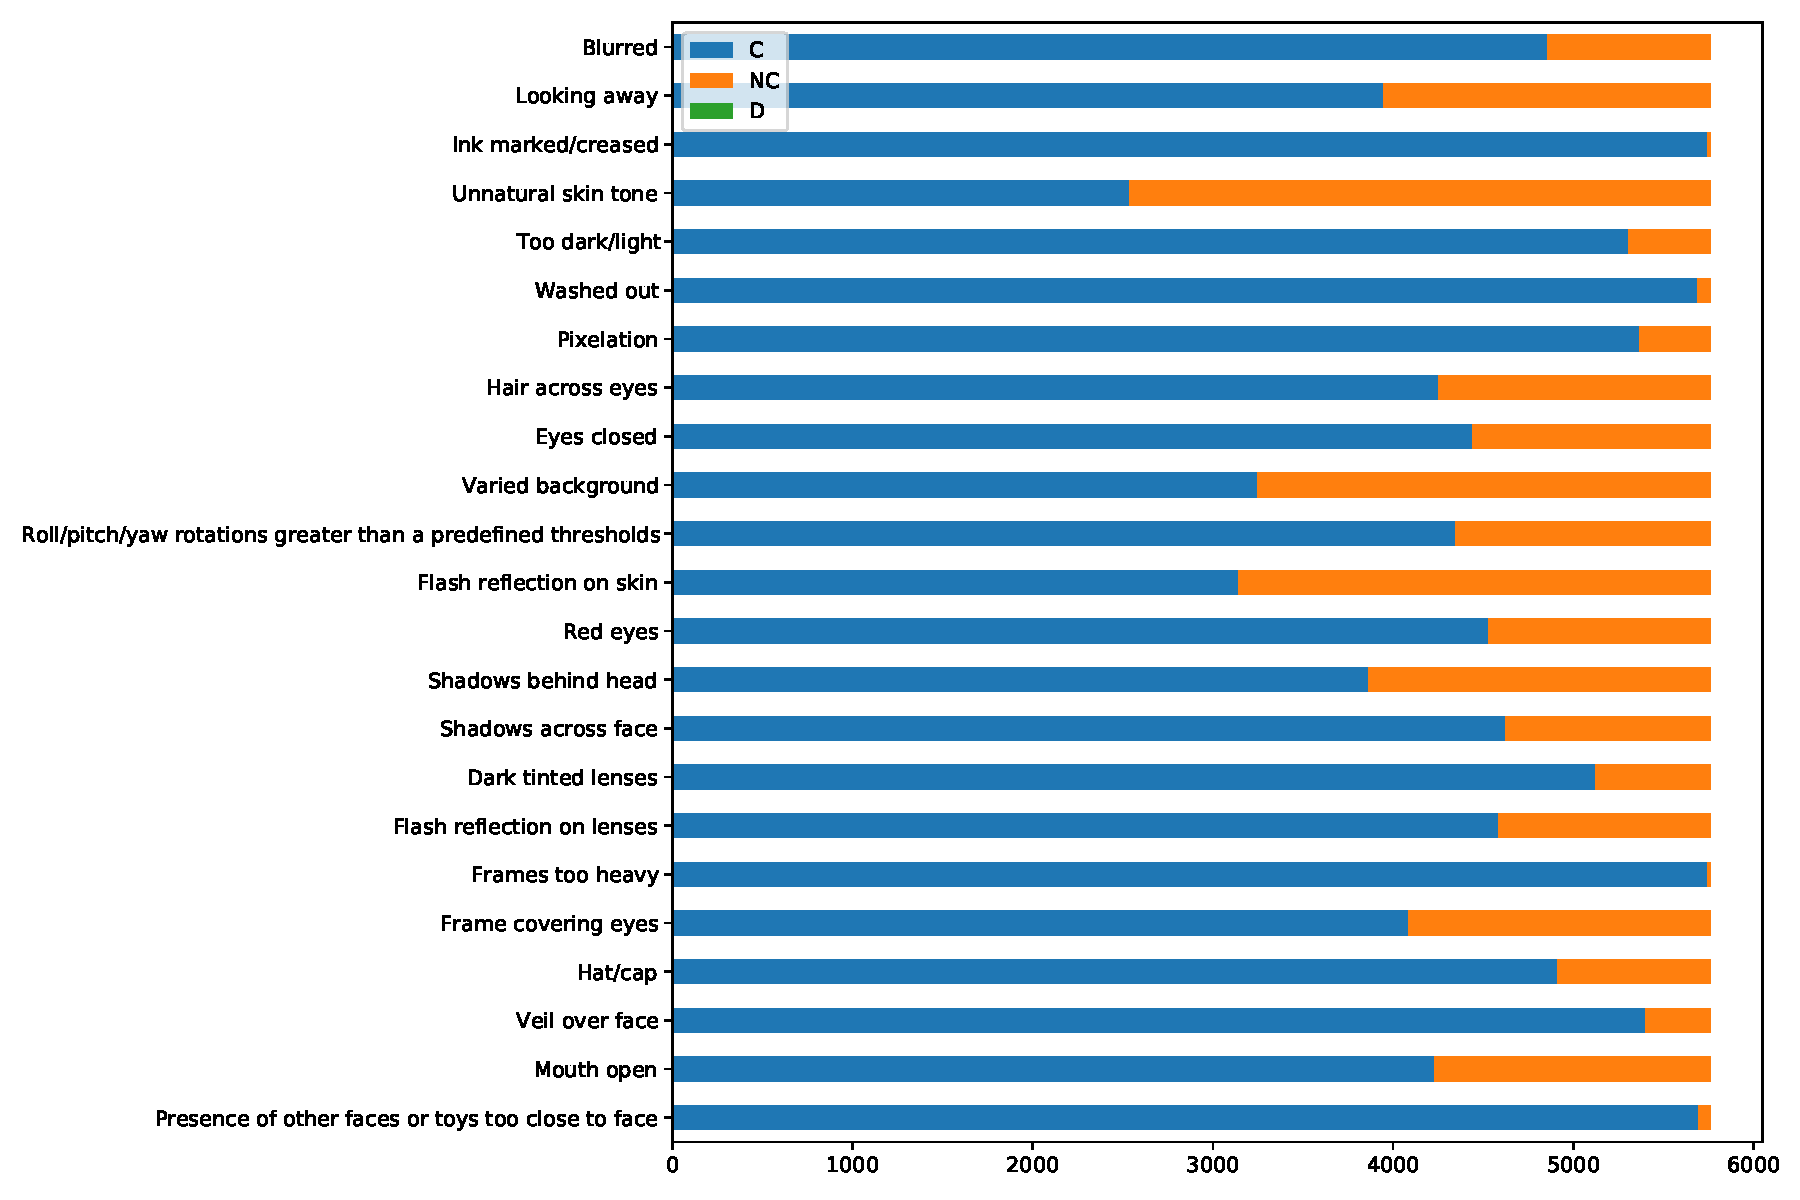
\includegraphics[width=\linewidth]{images/reqs_distribution.pdf}
\caption{Labels distribution per requirement. Source: own elaboration.}
\label{fig:reqs_distribution}
\end{figure*}

\autoref{fig:reqs_correlation} shows the correlation between non-compliant requirements. In other words, it measures how many images has two different non-compliant requirements occurring together. As expected, we can notice a strong correlation between eyes-related characteristics, e.g., \lookingaway, \hairacrosseyes, \eyesclosed, \redeyes, \darktintedlenses, and \framecoveringeyes. These are mainly caused by the dummy requirements that were converted to non-compliant. Moreover, considerable correlations can be observed between requirements associated to skin, for instance \unnaturalskintone and \flashskin. 

\begin{figure*}
\centering
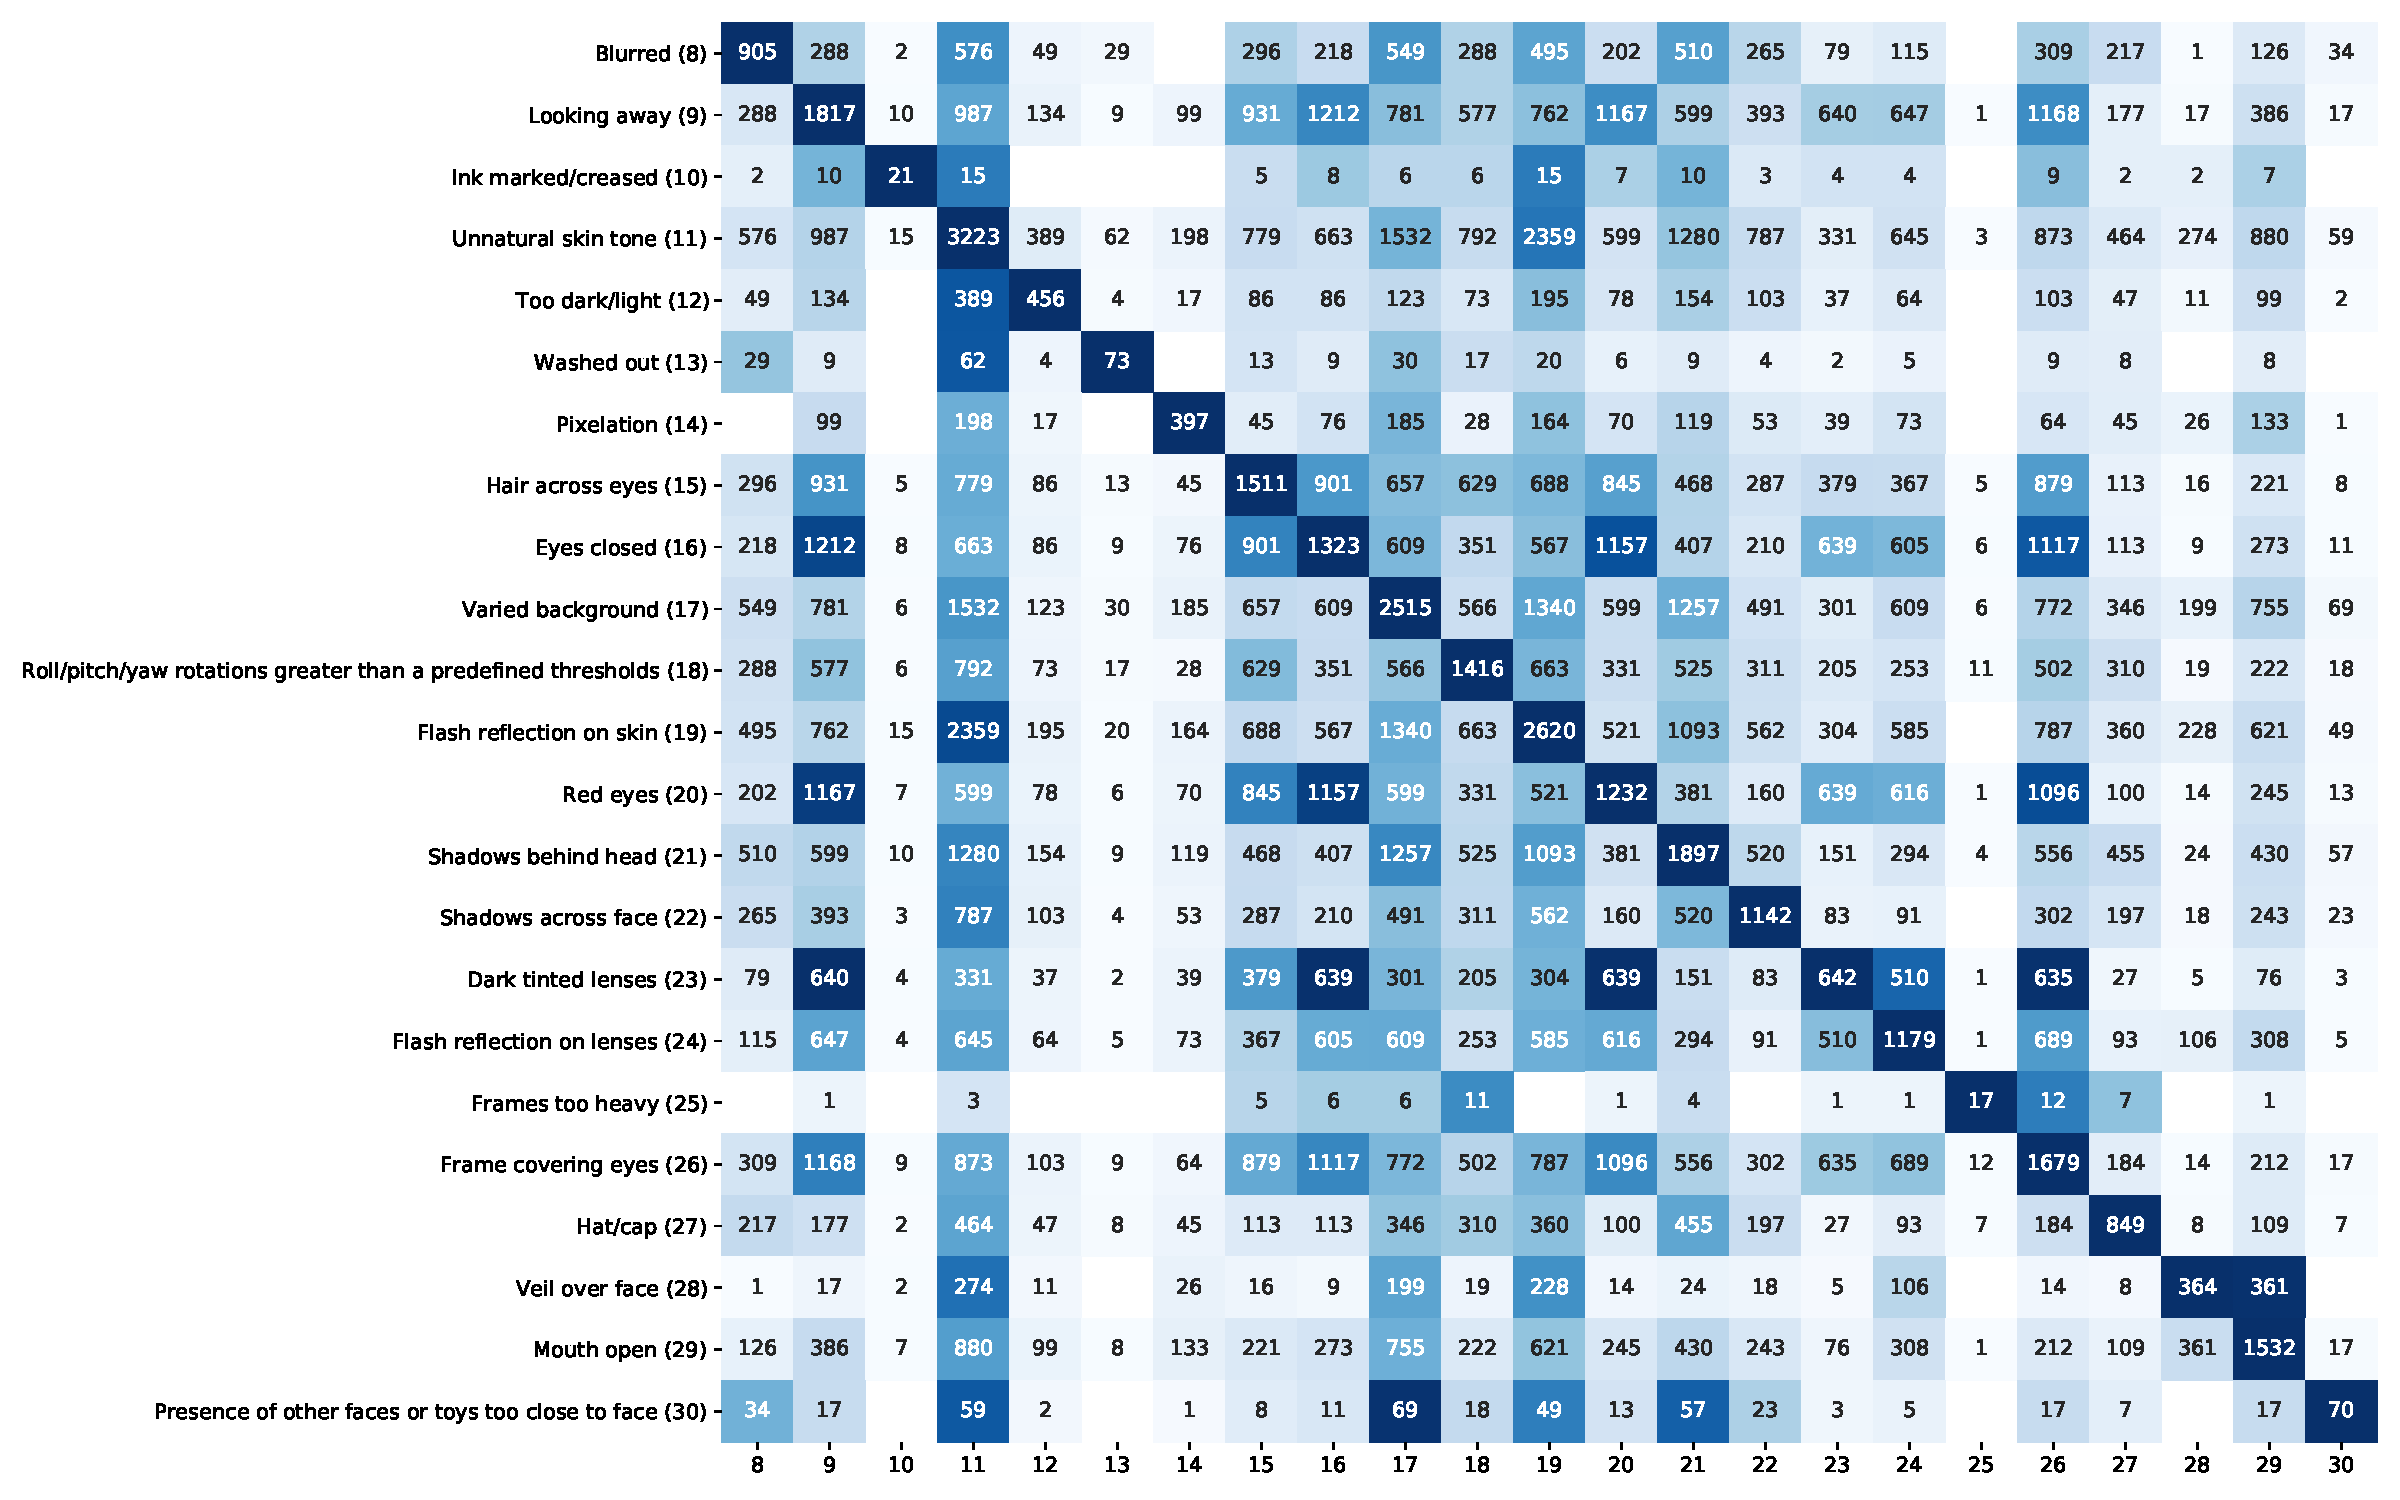
\includegraphics[width=\linewidth]{images/reqs_correlation.pdf}
\caption{Correlation between non-compliant requirements. Source: own elaboration.}
\label{fig:reqs_correlation}
\end{figure*}

According to our analysis, we came up with some conclusions. Firstly, since the dimensions of the images are different across the dataset, an approach to normalize images is required. It must avoid undesired normalization effects (like blur and pixelation) whenever possible and consider the trade-off between the input image quality and processing speed by the network. Regarding labels, the proposed method must consider the dataset unbalancing, and the most unbalance requirements might need special attention. Furthermore, the correlation between some requirements can be leveraged by a mechanism that shares features, like Autoencoders.

In the next section, we describe in detail the proposed method, called \methodname. It includes the architecture, the training process, as well the implementation details.

\subsection{\methodname}

\methodname is a \acl{dnn} developed to address the \icao standard. The architecture of \methodname is mainly based on Autoencoders. However, it is extended to apply a multi and collaborative learning approach. More details about the proposed method are described in the rest of this section. 

\subsubsection{Preprocessing} \label{sec:preprocessing}

Since the \adhoc dataset images have an extensive range of size dimensions (from 362$\times$362 to 4608$\times$3456 pixels), a preprocessing step was required to standardize the input image to \methodname. \autoref{fig:preprocessing} summarizes the preprocessing method applied in this work. A detailed explanation is provided as follows.

\begin{figure}
\centering
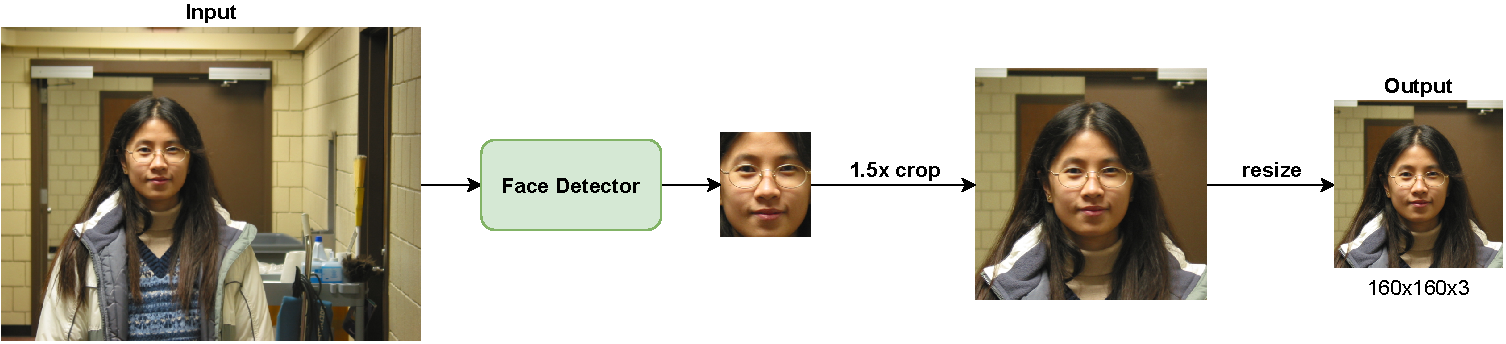
\includegraphics[width=\linewidth]{images/preprocessing.pdf}
\caption{Preprocessing step of \methodname. Source: own elaboration.}
\label{fig:preprocessing}
\end{figure}

The first step of our preprocessing method is face detection. We use a single shot multi-box detector based on MobileNet \citep{yeephycho} and trained on the WIDER FACE dataset \citep{yang2016wider}. This face detector has been chosen because it has a fair balance between speed and accurate results. According to our benchmarks, it was able to detect 98.99\% of all faces with an average processing time of 1.6s per image in CPU. Moreover, this detector is compatible with TensorFlow 1.X versions used by the proposed method. 

Since the bounding box of the detected face is limited to the face region (from forehead to chin), we crop a squared region 1.5$\times$ larger than the detected face to include background and other relevant information to assess the requirements. Padded regions are filled with zeros because it generates less undesired artifacts than methods like border reflection, replication, or wrap. We do not apply any image normalization like illumination correction or rotation as it can affect requirements evaluation. 

Finally, the cropped image is resized to 160$\times$160 pixels using the \texttt{INTER\_AREA} method of OpenCV\footnote{\url{https://docs.opencv.org/3.4/da/d54/group__imgproc__transform.html}}, since it is the recommended method for image decimation. Then, all pixels intensities are normalized to the real valued $[0...1]$ range before feeding to \methodname. Again, the size of 160$\times$160 was chosen considering the trade-off between speed and results. More details are provided in Chapter \ref{sec:results}. 

\subsubsection{Architecture}

The overall architecture of \methodname can be seen in Figure \ref{fig:icaonet}. The architecture is composed of an Autoencoder in combination with a dense network branch. While the Autoencoder is employed for unsupervised learning of a highly discriminative embeddings space, the dense layer performs multi-label classification. 

\begin{figure*}
\centering
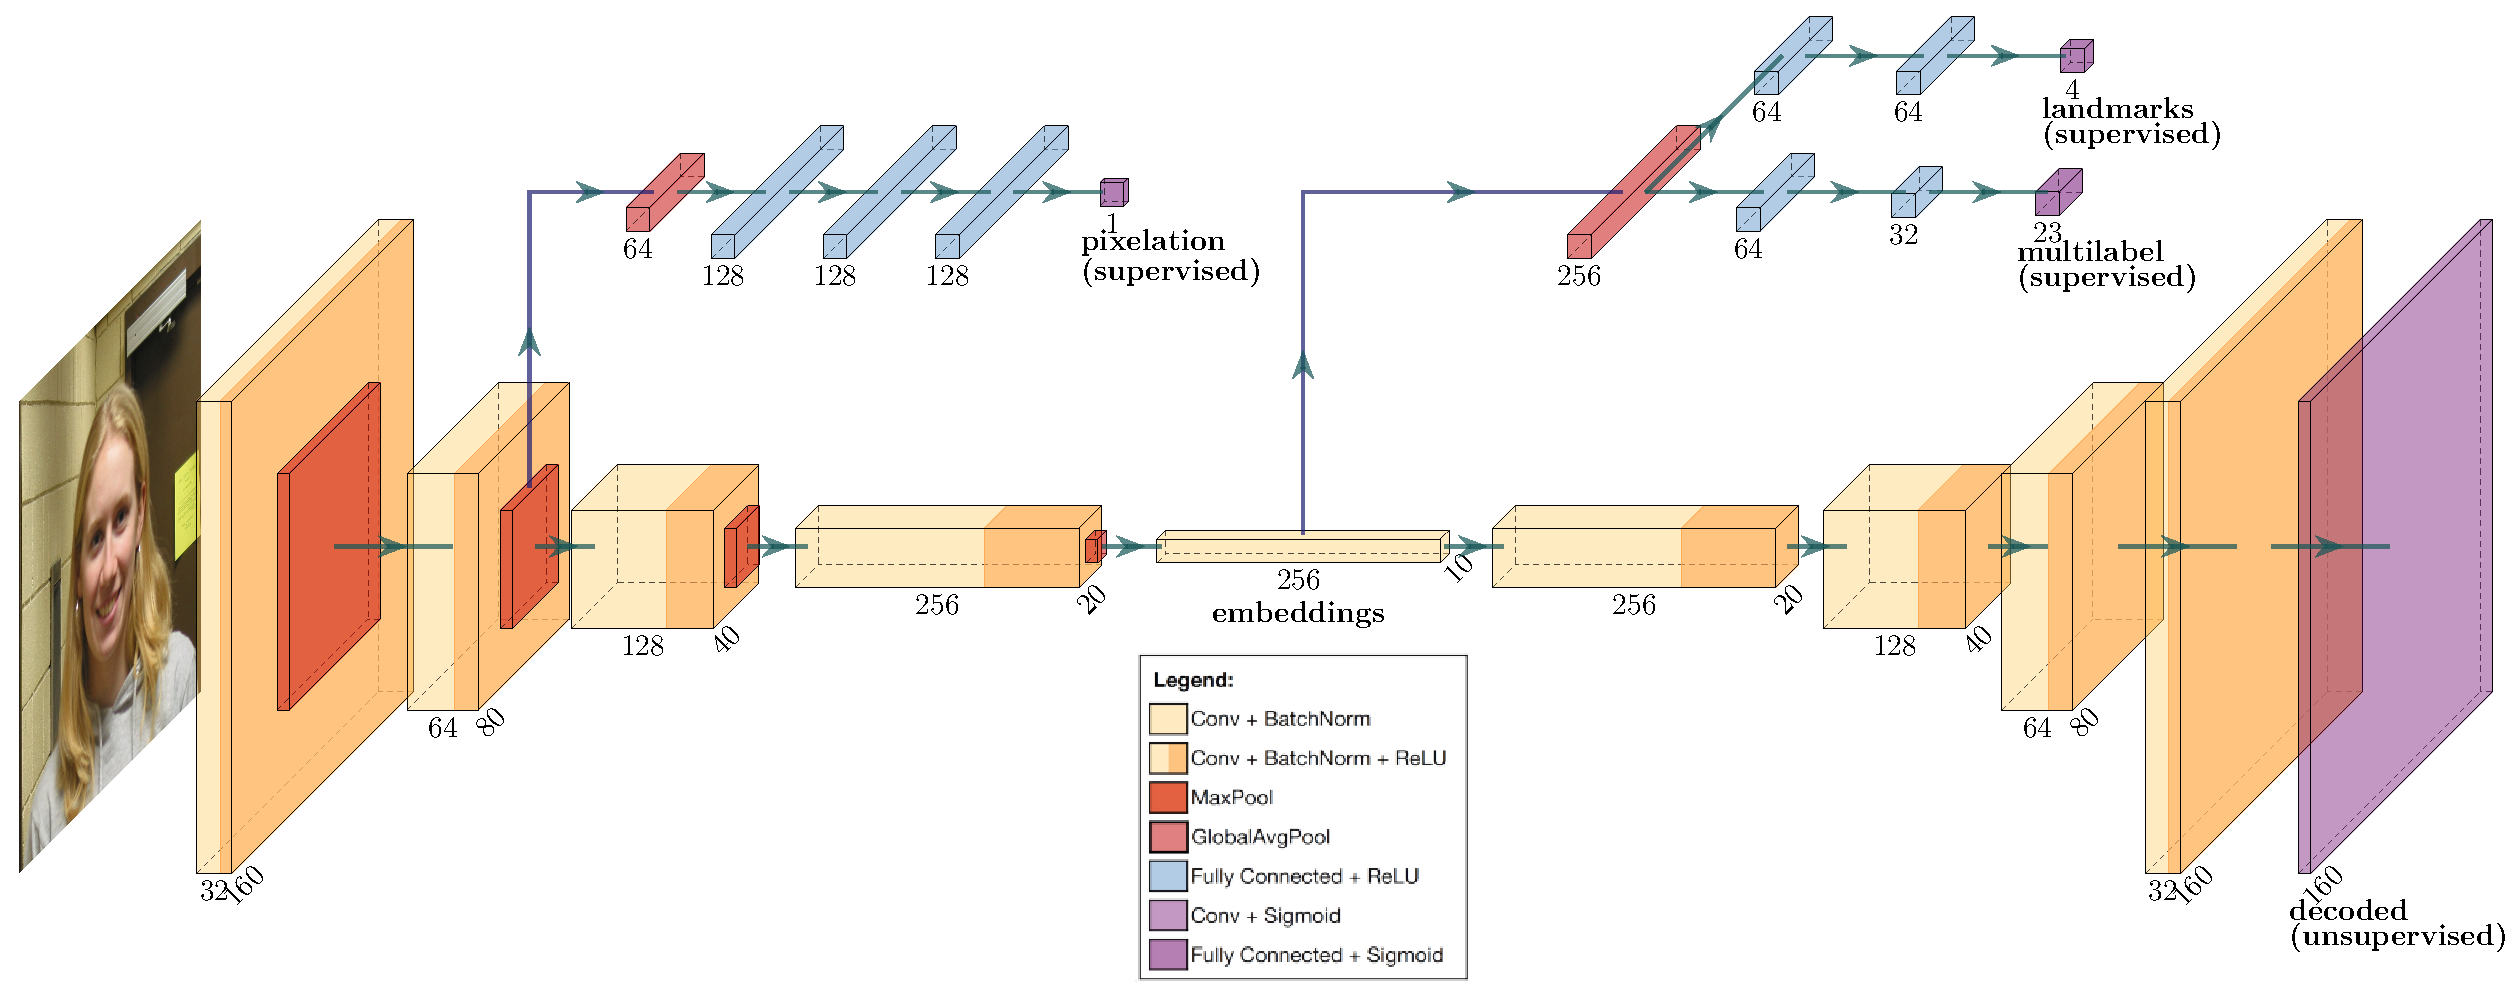
\includegraphics[width=\linewidth]{images/icaonet.pdf}
\caption{Architecture of \methodname. Source: own elaboration.}
\label{fig:icaonet}
\end{figure*}

The main idea behind the proposed architecture is to employ a multi and collaborative learning approach for the \icao requirements. It is multi-learning (also called multitasking) because the network solves both regression (image reconstruction) and multi-label classification (compliance prediction for each requirement) tasks at the same time. In contrast to \acfp{gan}, since both tasks are optimized together in training time, the learning process must also be collaborative. Hence, both branches must collaborate to learn an appropriate representation to solve both tasks. Additionally, we can assign different weights for each task to determine their importance during the optimization step (more details are given later).

The \methodname has three main components: (i) a \textbf{Shared Network} to compute shared embeddings; (ii) an \textbf{Unsupervised Branch} to perform image reconstruction; and (iii) a \textbf{Supervised Branch} for requirements assessment. Such components are detailed as follows.

\paragraph{Shared Network}

The initial part of the network is responsible for learning the embeddings shared by the unsupervised and supervised branches. These embeddings can be interpreted as a proper representation of the input and can be defined as an encoder function $h = f(x)$. Besides being used for dimensionality reduction, the shared embeddings are also used for feature learning in our network.

The architecture to compute the shared embeddings is based on the encoder component of Undercomplete Convolutional Autoencoder networks \citep{goodfellow2016deep}. The supervised branch receives a preprocessed input image of size 160x160 pixels in the BGR color channel. Details of the preprocessing are given in Section \ref{sec:preprocessing}. The first four convolutional layers are composed of 3x3 filters with batch normalization and ReLU activation. A 2D Max-pooling layer is applied for dimensionality reduction after each layer. The fifth layer is also composed of 3x3 convolutions with batch normalization. However, $tanh$ is used as a non-linear activation function instead of ReLU to normalize the embeddings values between -1 and 1. In our experiments, $tanh$ performed slightly better than ReLU for the encoded representations. The output of this layer stores the embeddings shared by the other branches. The embeddings are a 256-dimensional vector.

\paragraph{Unsupervised Branch}

This branch represents the decoder of an Autoencoder network. It is responsible for decoding the shared embeddings back to the original input. In mathematical terms, this branch will be responsible to learn the decoder function $\hat{x} = g(h)$, where $\hat{x}$ represents the reconstructed image. 

The architecture reflects the first four convolutional layers of the shared embeddings network. However, the Max-pooling layers are replaced by 2D Transposed Convolution layers. Furthermore, the last layer activation function is sigmoid since the input image pixels are normalized into the $[0...1]$ range. The shared embeddings network, together with the unsupervised branch, produces a full Convolutional Autoencoder Network \citep{goodfellow2016deep}.

The unsupervised branch uses the Mean Squared Error (MSE) to measure the image reconstruction task ($\mathcal{L}_1$), as defined by \autoref{eq:loss-unsupervised}:

\begin{equation}
\label{eq:loss-unsupervised}
\mathcal{L}_1 = \frac{1}{N} \sum_h^H \sum_w^W ({I_{h,w} - \hat{I}_{h,w}})^2
\end{equation}

\noindent where $N$ represents the number of pixels; $H$ and $W$, the image dimensions; $I$ and $\hat{I}$ are the input image and the reconstructed image, respectively. Since the same input image $I$ is used in the reconstruction task as a ground-truth, this task is considered unsupervised (sometimes also called semi-supervised). During training, the unsupervised branch will minimize the squared difference between the input image $I$ and the reconstructed image $\hat{I}$.

\paragraph{Supervised Branch}

This branch takes the shared embeddings as input and applies a fully connected network to perform multi-label classification. The first layer of this branch performs a GlobalAveragePooling to the shared embeddings. It transforms the 4-D dimensional vector of the embeddings into 2-D dimensions required by dense networks. We chose GlobalAveragePooling layers instead of Max Pooling layers since they are known to perform better in practice, as stated in \cite{zhou2016learning}. Then, there are two consecutive dense layers with 64 and 32 neurons, respectively. Dropout layers are included between each layer to prevent overfitting. Finally, the output layer has 23 neurons with sigmoid activation. Therefore, each neuron of the final layer outputs a normalized score between 0 and 1 for each corresponding requirement. In practice, the supervised branch's output is considered the likelihood of a given input image being compliant to each requirement of \icao standard.

We compute the Multi-label Cross-Entropy as the loss function for the supervised branch, defined by \autoref{eq:loss-supervised}:

\begin{equation}
\label{eq:loss-supervised}
\mathcal{L}_2 = \frac{1}{M} \sum_i^M {y_i \cdot log(\hat{y}_i)}
\end{equation}

\noindent where $M$ represents the number of requirements; $y_i$ is the ground-truth for each requirement (0: non-compliant, 1: compliant); and $\hat{y}_i$ is the predicted score for each requirement.

Since the network has two branches (supervised and unsupervised) and they are optimized using two different loss functions ($\mathcal{L}_1$ and $\mathcal{L}_2$), the final loss function $\mathcal{L}(I, \hat{I}, y, \hat{y})$ is defined by the \autoref{eq:loss-final}:

\begin{equation}
\label{eq:loss-final}
\mathcal{L}(I, \hat{I}, y, \hat{y}) = \lambda\mathcal{L}_1 + \gamma\mathcal{L}_2
\end{equation}

\noindent where $\lambda$ and $\gamma$ are two hyperparameters to control the trade-off between each loss function.

\subsubsection{Training} 

To train \methodname, the \ficvtest dataset is split into training and validation sets only. We consider the private dataset of the FICV competition (\ficvofficial) as the test set, and the benchmark results are reported as our final results. Both training and validation sets are randomly divided using a stratified multi-label approach. Thus, the compliant and non-compliant proportions seen in Table \ref{tab:req-dist} are preserved. Approximately 10\% of the dataset (580 images) is used as the validation set, while the remaining images are selected for network training.

Regarding the architecture, since most of the \methodname structure is based on undercomplete Autoencoders, there was no need to employ many regularization techniques during training. However, we still apply batch normalization before activation functions in the Convolutional layers and Dropouts in some dense layers of the supervised branch. The Early Stopping technique is also employed to prevent overfitting, and the patience hyperparameter is based on the \acf{mcc}, as presented in \autoref{eq:mcc}. The MCC was chosen because it is a robust metric for unbalanced datasets (see Section \ref{sec:mcc} of Chapter \ref{sec:background}) and it performed better than \acs{eer} in our experiments. All metrics described in Section \ref{sec:measures} of Chapter \ref{sec:background} are evaluated at the end of each epoch and will be reported in the results chapter.

The network is written in Python using Keras\footnote{\url{https://keras.io}} framework (v2.3.1) with TensorFlow (v1.13.1) backend. The Mlflow\footnote{\url{https://www.mlflow.org}} library (v1.7.0) is used for experiments tracking/comparison and logging of hyperparameters, metrics, and artifacts. The source code, along with the trained network, can be found in Github\footnote{\url{https://github.com/arnaldog12/doutorado}}. Furthermore, the experiments are conducted in a Windows 10 machine with Intel\textsuperscript{\tiny\textregistered} Core\textsuperscript{\tiny\texttrademark} i5-8300H of 8\textsuperscript{th} generation, 16 GB of DDR4 2666MHz RAM, SSD of 512 GB, and NVIDIA\textsuperscript{\tiny\textregistered} GeForce\textsuperscript{\tiny\textregistered} GTX 1050 with 4GB of RAM.

One last important detail about \methodname training is that we took special care over the experimentation phase. For example, we set the random seed of Python, its \texttt{random} module\footnote{\url{https://docs.python.org/3/library/random.html}}, and Numpy\footnote{\url{https://numpy.org}} and TensorFlow libraries to be the same for all experiments. It assures reproducibility and ensures that the best results of current experiments are not achieved by chance.

\subsubsection{Parameters and Hyperparameters} \label{sec:hyperparams}

The base architecture of \methodname -- composed of the three components described earlier (shared network, supervised branch, and unsupervised branch) -- contains a total of 1,980,890 parameters. From these parameters, 1,978,458 are trainable, and the remaining 2,432 are non-trainable parameters related to the mean and variance computed by batch norm layers. In terms of size, the \methodname occupies 22.8 MB in the disk when stored as a \texttt{.hdf5} file.

One important detail to mention about the proposed architecture refers to the unsupervised branch, which is used during training only. Once the network is trained, the unsupervised branch is detached from the model as the reconstruction task is not valuable for ICAO assessment and can be ignored. In this case, the number of parameters is reduced to 1,000,727. Furthermore, after model \textit{freezing}\footnote{Freezing is a typical operation in Keras/TensorFlow models. It removes unnecessary data for prediction in the model file, e.g., the optimizer, metrics, metadata, gradients, and many others. It may not be confused with layer freezing.}, the model size is reduced to only 3.83 MB in the disk. It helps speed up the running time considerably.

The \methodname was trained by 100 epochs and a batch size of 32. All layers are randomly initialized by Xavier initialization \citep{glorot2010understanding}. To prevent overfitting and improve generalization, we use Early Stopping with 30 epochs of patience. In layers where Dropout is applied, we keep 50\% of neurons. The Adaptive Momentum Estimation (Adam) is applied as optimizer with learning rates $\alpha=10^{-3}$, $\beta_1=0.9$, $\beta_2=0.999$, and $\epsilon=10^{-7}$. For the loss function (\autoref{eq:loss-final}), we use $\lambda=1.0$ and $\gamma=2.0$.
